\section{Experiment design}\label{sec:experiment_design}
%Forsoegsopstilling, der inkludere en tegning af omraadet set oppefra med indtegning af beacons, objectern og hvor rigtige position for test person.
Experiments for the evaluation of the implemented system are carried out in an n times n meeting room.
In the room, a partition and a cabinet are placed between two tables, effectively dividing a single meeting room into two smaller areas. 
In each of the smaller areas a table with six chairs is placed and on the walls are placed whiteboards.
\begin{figure}[h]
    \centering
    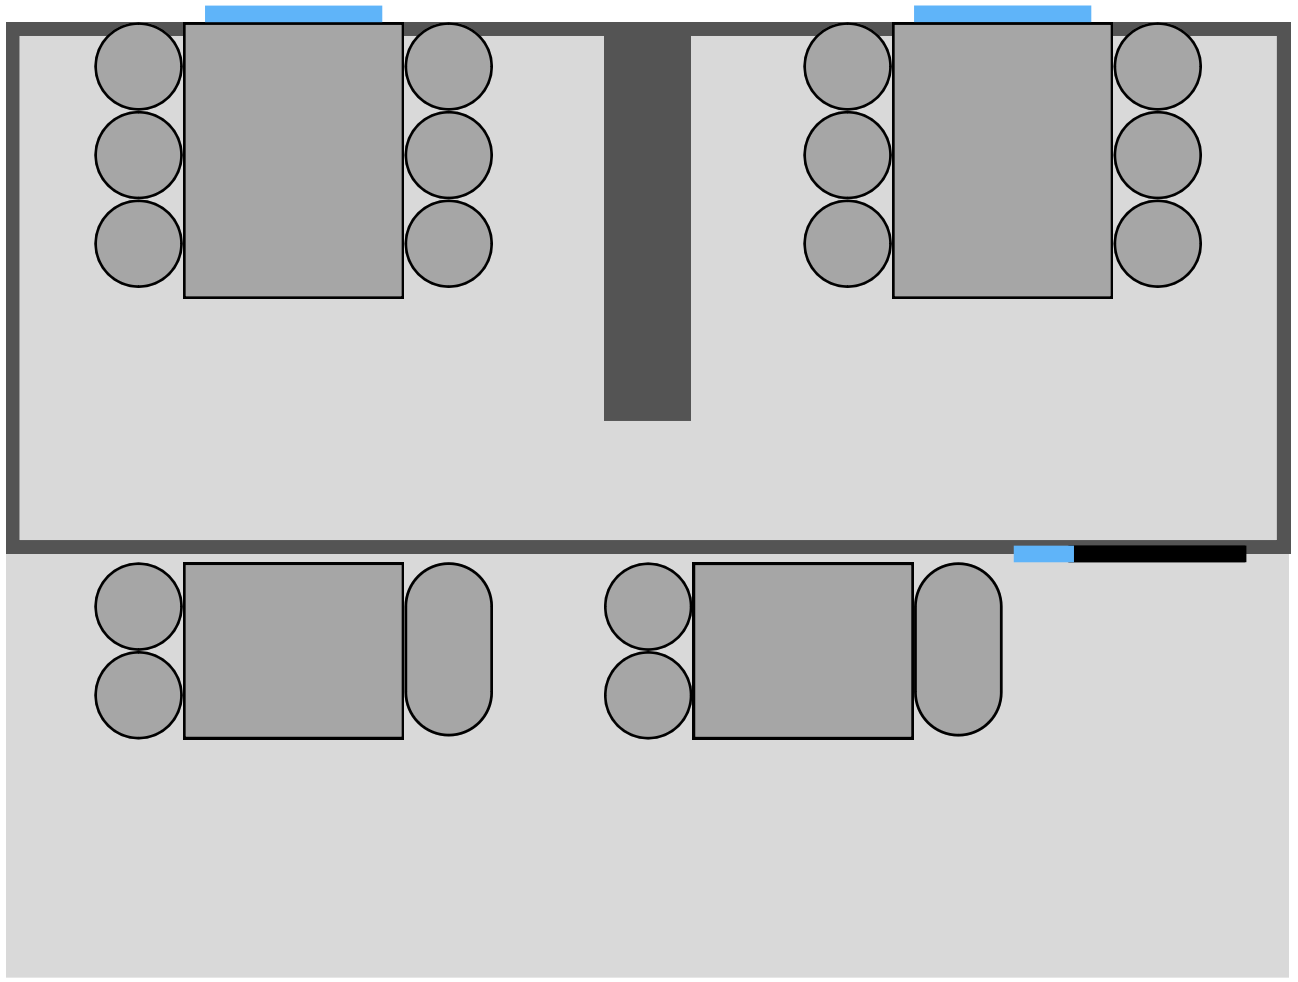
\includegraphics[scale=0.7]{images/experiment_room.png}
    \caption{The meeting room in which the experiments were carried out.}
    \label{fig:experiment_room}
\end{figure}
On one end of each table is a large, rectangular window.
Furthermore, one table has a large TV screen placed near the window. 
Near the door of the room, an airconditioning controller and a large glass window are located.
Lighting is built into the ceiling, thus no hanging light will interfere with the broadcasted signals. 
Outside the meeting room is a common area.
This area contains two high tables.
Each of these tables has a small couch and two chairs placed next to it.
Beacons are placed on top of the cabinet and in the three corners furthest away from the door.   
The meeting room and its surrounding area is depicted in Figure \ref{fig:experiment_room}.
\begin{figure}[h]
    \centering
    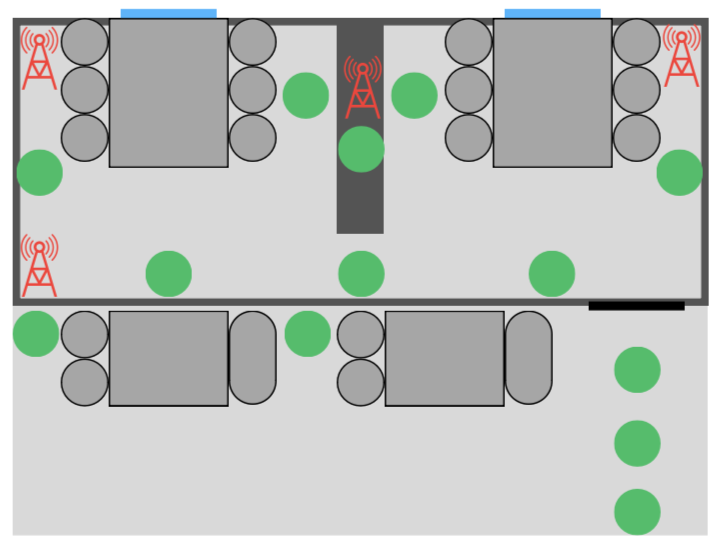
\includegraphics[scale=0.7]{images/experiment_setup.png}
    \caption{The meeting room in which the experiments were carried out, decorated with beacon placements (red antenna) and measurement locations(green circles)}
    \label{fig:experiment_setup}
\end{figure}
When performing the evaluations, we want to examine whether the system can correctly classify whether a receiving device is inside the room.
We do this by performing measurements inside, outside, and on borders of the room.
As physical obstacles can cause fluctuations in the received signals, we design the expirement such that measurements are takens in areas where some, none, and all of the beacons are blocked. 
We perform measurements in the following areas:
\begin{itemize}
    \item Along the walls inside of the meeting room
    \item Along both sides of the divider
    \item On the cabinet, next to the beacon
    \item 1m, 2m, 5m outside the door
    \item By the tables in the common area. 
\end{itemize}
The experimental set up is seen in Figure \ref{fig:experiment_setup}.




%room description

